\documentclass{standalone}
\usepackage{tikz}
\usepackage{ctex,siunitx}
\setCJKmainfont{Noto Serif CJK SC}
\usepackage{tkz-euclide}
\usepackage{amsmath}
\usetikzlibrary{patterns, calc}
\usetikzlibrary {decorations.pathmorphing,decorations.pathreplacing,decorations.shapes,}
\begin{document}
\small
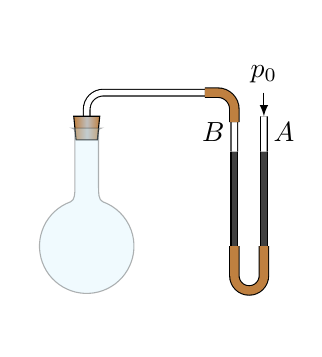
\begin{tikzpicture}[>=latex,scale=0.75]
  \useasboundingbox(-1.0,-1.4)rectangle(3.5,3.7);
  \draw[double,double distance=2pt,rounded corners=6pt](0,2.0)--(0,2.6)--(2.5,2.6)--(2.5,1.6)(3.0,1.6)--(3.0,2.2);
  \draw[double=darkgray,double distance=2pt](2.5,1.6)node[above left]{$B$}--(2.5,0)(3.0,1.6)node[above right]{$A$}--(3.0,0);
  \draw[double=brown,double distance=3pt](2.5,0)--++(0,-0.5)arc(180:360:0.25)--++(0,0.5);
  \draw[double=brown,double distance=3pt,rounded corners=6pt](2.0,2.6)--(2.5,2.6)--(2.5,2.1);
  \draw[left color=brown,right color=brown,middle color=lightgray](-0.18,1.8)--(-0.22,2.2)--(0.22,2.2)--(0.18,1.8)--cycle;
  \draw[fill=cyan!20,opacity=0.3](0,2.0)--(-0.25,2.0)arc(90:0:0.05)--(-0.2,1)..controls(-0.2,0.9)and(-0.2,0.7785)..(110:0.8)arc(110:430:0.8)..controls(0.2,0.7785)and(0.2,0.9)..(0.2,1)--(0.2,1.95)arc(180:90:0.05)--cycle;
  \draw[thin,->](3,2.6)--++(0,-0.4)node[at start,above]{$p_0$};
\end{tikzpicture}
\end{document}